\documentclass{article}
\usepackage{graphicx}
\usepackage{subcaption}
\usepackage{listings}
\usepackage{color}
\usepackage{hyperref}
\usepackage{amsmath}

\renewcommand\lstlistingname{Quelltext} % Change language of section name

\lstset{ % General setup for the package
	language=Perl,
	basicstyle=\small\sffamily,
	numbers=left,
 	numberstyle=\tiny,
	frame=tb,
	tabsize=4,
	columns=fixed,
	showstringspaces=false,
	showtabs=false,
	keepspaces,
	commentstyle=\color{red},
	keywordstyle=\color{blue}
}
\pagenumbering{arabic}
\begin{document}

\begin{titlepage}
	\centering
	
\includegraphics[width=0.4\textwidth]{irif_horizontal}
	
\includegraphics[width=0.4\textwidth]{Logo80ANS_OR}\par\vspace{1cm}
	
\includegraphics[width=0.4\textwidth]{logop7}
	
\includegraphics[width=0.4\textwidth]{Universite_Paris_logo_horizontal}\par\vspace{1cm}
	{\scshape\LARGE Université Paris Diderot \par}
	{\scshape\Large -\par}

	{\scshape\LARGE IRIF \par}
	\vspace{1cm}
	{\scshape\Large Rapport de Stage\par}
	{\scshape\Large du 01/06/2019 au 01/08/2019\par}
	\vspace{1.5cm}
	{\scshape\Large éffectué à Paris\par}
	\vspace{1.5cm}
	{\Large\itshape Sébastien Lecleire\par}
	{\Large\itshape Etudiant en MASTER 1 IMPAIRS\par}
	\vfill
	supervisé par\par
	Mr Yann \textsc{Régis-Gianas}

	\vfill
\end{titlepage}


\newpage

\tableofcontents
\newpage

\section{Remerciements}
Avant tout développement sur cette expérience professionnelle, il apparaît opportun de commencer ce rapport de stage par des remerciements, à ceux qui m’ont beaucoup appris au cours de ce stage, et même à ceux qui ont eu la gentillesse de faire de ce stage un moment très profitable.
\newline
Tout d'abord, j'adresse mes remerciements à ma professeure et amie, Mme Ines Klimann, maître de conférences à l'Université Paris Diderot (Paris 7) qui m'a beaucoup aidé dans ma recherche de stage.
\newline
Je tiens à remercier vivement mon maitre de stage, Mr Yann Régis-Gianas, maître de conférences à l'Université Paris Diderot (Paris 7) et responsable de la platforme LearnOCaml au sein de l'IRIF pour son accueil, son enthousiasme et ses conseils avisés. Grâce à sa confiance j'ai pu accomplir mes différentes missions en totale autonomie avec rigueur et efficacité. Il fut d'une aide précieuse dans les moments les plus délicats.
\newline 
Je remercie également l'ensemble des employés de l'IRIF et de l'Université Paris Diderot (Paris 7) pour leur accueil, leur gentillesse et leur professionnalisme.
Enfin, je tiens à remercier toutes les personnes qui m'ont conseillé et aidé lors de mon stage.


\newpage

\section{Introduction}

Du 01/06/2019 au 01/09/2019, j’ai effectué un stage au sein de l'Institut de Recherche en Informatique Fondamentale (IRIF\footnote{\label{IRIF} Institut de Recherche en Informatique Fondamentale}). Au cours de ce stage dans l'équipe \begin{math}\pi r^2\end{math}, j’ai pu m’intéresser au développement des méthodes formelles ou mathématiques pour modéliser des systèmes existants, naturels ou artificiels, et pour résoudre des problèmes concrets.
Plus largement, ce stage a été l’opportunité pour moi d’appréhender l'aspect pratique de tous les metiers liés au développement d'une application de sa conception à sa mise en production des méthodes pour rendre plus sûre et plus efficace la distribution de systèmes logiciels de grande dimension.
\newline\newline
Au-delà d’enrichir mes connaissances informatiques, ce stage m’a permis de comprendre énormement de chose sur le travail en équipe, sur les subtilités de la vie en entreprise et m'a donné de nombreuses pistes sur mon orientation après mon Master 2.
Mon stage au pôle Preuves, Programmes et Systèmes (PPS\footnote{\label{PPS} Preuves, Programmes et Systèmes}) de l'IRIF\ref{IRIF} a consisté essentiellement en l'amélioration de la platforme LearnOCaml et au développement d'applications permettant de faciliter et de simplifier son utilisation.
Mon maître de stage étant maître de conférences à l'Université Paris Diderot (Paris 7) et membre permanant du pôle PPS\ref{PPS}, j’ai pu apprendre dans d’excellentes conditions à utiliser de nombreux outils mis à disposition par Github et à réaliser un FrontEnd, un BackEnd, une API\footnote{\label{API} Interface de Programmation d’Application ou Interface de Programmation Applicative}, à administrer des serveurs Cloud Openstack et des Nodes Kubernetes aussi bien en local qu'avec OVH.
\newline\newline
Ce stage a donc été une opportunité pour moi de percevoir comment les recherches menées à l'IRIF\ref{IRIF} reposent sur l’étude et la compréhension des fondements de toute l’informatique, afin d’apporter des solutions innovantes aux défis actuels et futurs des sciences numériques.
L’élaboration de ce rapport a pour principale source les différents enseignements tirés de la pratique journalière des tâches auxquelles j’étais affecté.
\newline\newline
En vue de rendre compte de manière fidèle et analytique des 2 mois passés au sein de l'IRIF\ref{IRIF}, il apparaît logique de présenter à titre préalable le cadre du stage : l'IRIF\ref{IRIF}, et l’environnement du stage, à savoir le secteur PPS\ref{PPS}. Ensuite, il sera précisé les différentes missions et tâches que j’ai pu effectuer au sein du pôle PPS\ref{PPS}. Enfin les nombreux apports que j’ai pu en tirer.

\newpage

\section{L'IRIF}

L'Institut de Recherche en Informatique Fondamentale (IRIF) est une unité mixte de recherche (UMR 8243) entre le CNRS et l'université Paris Diderot, qui héberge deux équipes-projets INRIA. Il est issu de la fusion des deux UMR LIAFA et PPS au 1er janvier 2016. L'IRIF est aussi membre de la Fondation Sciences Mathématiques de Paris (FSMP). 

\subsection{Présentation}

l’IRIF est reconnu pour ses contributions portant sur la conception et l’analyse d’algorithmes, l’étude des modèles de calculs et de représentation des données, les fondements des langages de programmation, le développement logiciel, la vérification et la certification. L’IRIF effectue aussi une recherche interdisciplinaire mettant à profit sa démarche scientifique.
\newline\newline
L’IRIF s'appuie sur des concepts mathématiques développés et étudiés en son sein, notamment en combinatoire, théorie des graphes, logique et algèbre. Ces travaux contribuent aussi directement aux mathématiques, notamment en physique combinatoire, probabilités, catégories, théorie de la preuve, et preuves assistées par ordinateur.
\newline\newline
Au CNRS, l'IRIF est principalement rattaché à l'Institut National des Sciences de l'Information et de leurs Interactions (INS2I) et, secondairement, à l'Institut National des Sciences Mathématiques et de leurs Interactions (INSMI). L'IRIF est membre de l'UFR d'informatique de l'université Paris Diderot, et accueille également en son sein plusieurs membres de l'UFR de mathématiques. Enfin, l'IRIF est associé à l'école doctorale des Sciences Mathématiques de Paris Centre (ED 386).
\newline\newline
L'IRIF est structuré en neuf équipes thématiques regroupées en trois pôles de recherche :
	\begin{itemize}
		\item[$\ast$]Pôle Algorithmes et structures discrètes
		\item[$\ast$]Pôle Automates, structures et vérification
		\item[$\ast$]Pôle Preuves, programmes et systèmes
	\end{itemize}
L'IRIF compte actuellement une centaine de membres permanents, se répartissant environ en 48 enseignants-chercheurs, 27 chercheurs CNRS, 5 chercheurs INRIA, 8 membres émerites et 7 personnels administratifs ou techniques (en janvier 2019). L'effectif total de l'IRIF, incluant doctorants, postdoctorants, et visiteurs de longue durée s'élève à près de deux cents personnes.
\newline\newline
Six membres de l'IRIF ont été lauréats de l'European Research Council (ERC), trois sont membres de l'Institut Universitaire de France (IUF) et deux sont membres de l'Academia Europæa. 

\subsection{PPS}

Thèmes de recherche
\newline\newline
Le programme scientifique du pôle Preuves, programmes et systèmes (PPS) de l'IRIF vise à renforcer les fondements théoriques des langages de programmation, des assistants de preuves et, plus généralement, des formalismes de calcul. Ces problématiques sont abordées en croisant trois points de vue complémentaires :
\begin{itemize}	
	\item[$\ast$]une approche syntaxique, qui développe des langages théoriques issus de formalismes logiques
    \item[$\ast$]une approche algébrique, qui étudie les structures mathématiques liées au calcul
	\item[$\ast$]une approche pratique, qui modélise et analyse des systèmes de calcul réels
\end{itemize}
Le pôle est constitué de trois équipes thématiques, correspondant à chacun de ces trois points de vue. Elles développent leurs outils propres, et les mettent ensuite au service d'objectifs scientifiques communs :
\begin{figure}[h!]
	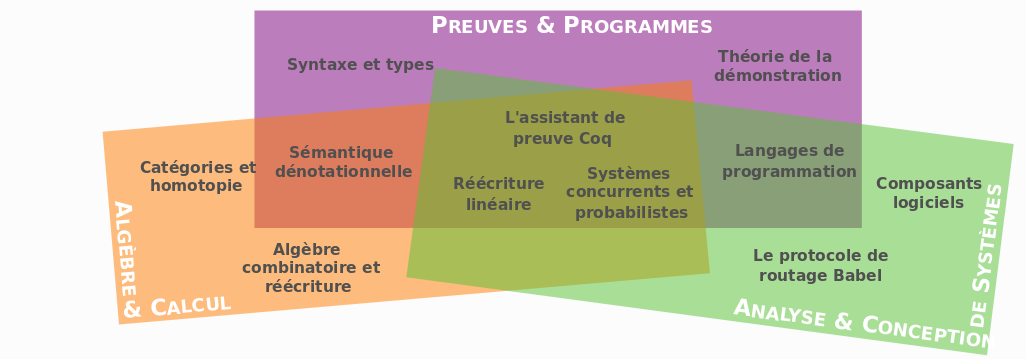
\includegraphics[width=\linewidth]{PPS.png}
	\caption{Diagramme des équipes PPS.}
\end{figure}
\newline
Le pôle PPS héberge l'équipe-projet \begin{math}\pi r^2\end{math} commune à l'INRIA, au CNRS et à l'Université Paris-Diderot — Paris 7, ainsi qu'une partie des membres de l'IRILL (Initiative de Recherche et d'Innovation sur le Logiciel Libre), une structure commune à l'INRIA, à l'Université Paris-Diderot — Paris 7 et à l'Université Pierre-et-Marie-Curie — Paris 6. 
\newpage
\section{Mes missions}

21. 
22. 

\subsection{les missions (responsabilités, tâches à effectuer, dossiers confiés, objectifs)}

\subsection{le bilan
résultats obtenus ( appréciation du maître de stage - productivité ... gestion du temps)
difficultés rencontrées et solutions apportées
enseignements/apports du stage (connaissances - compétences)}

\newpage

\section{Les apports du stage}
Merci !

\subsection{Subsection}

\newpage

\section{Conclusion}

Ce stage a été très enrichissant pour moi car il m’a permis de découvrir dans le détail le secteur du ………, ses acteurs, contraintes… et il m’a permis de participer concrètement à ses enjeux au travers de mes missions variées comme celle du …. que j’ai particulièrement apprécié. Ce stage m’a aussi permis de comprendre que les missions créatives n’étaient pas les plus adaptées pour moi…et je préfère m’orienter vers les métiers de …. qui me conviennent mieux.(Cette partie doit faire le bilan des plus et moins du stage / votre enrichissement pour votre future carrière)


L’entreprise … qui m’a accueilli pendant ce stage fait face à une période charnière…, et je suis très fier d’avoir pu contribuer, participer à cette révolution. L’évolution des usages et l’adaptation de l’entreprise au changement de son environnement….
(Cette partie doit montrer que vous avez su comprendre les enjeux économiques des secteurs de l’entreprise et/ou réponse à la problématique du rapport)


Fort de cette expérience et en réponse à ses enjeux, j’aimerai beaucoup par la suite essayer de m’orienter via un prochain stage, vers le secteur … avec des acteurs de petites tailles, et un important développement d’avenir.
(ouverture …prochaine étape)


\newpage
\section{Tests}
\begin{figure}[h!]
  \centering
  \begin{subfigure}[b]{0.2\linewidth}
    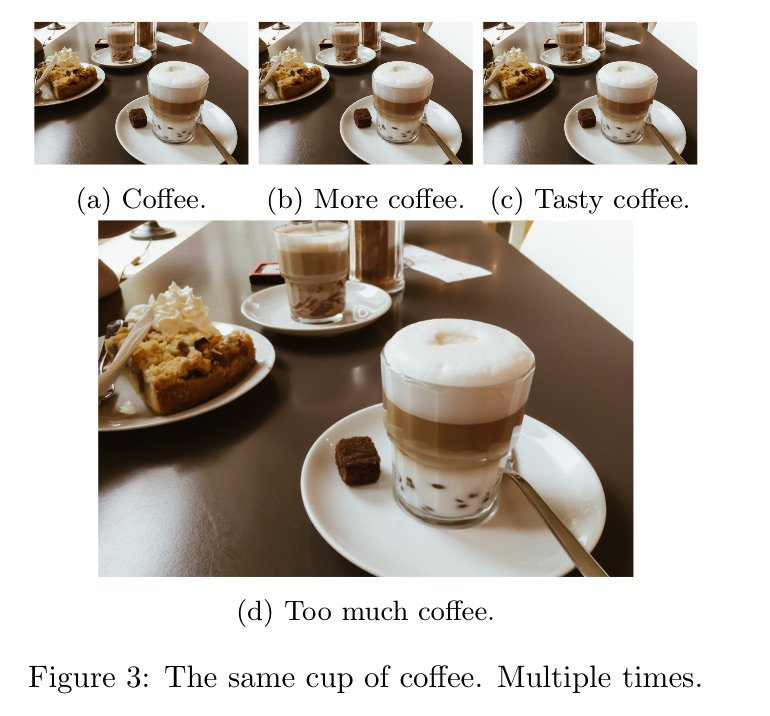
\includegraphics[width=\linewidth]{coffee.jpg}
     \caption{Coffee.}
  \end{subfigure}
  \begin{subfigure}[b]{0.2\linewidth}
    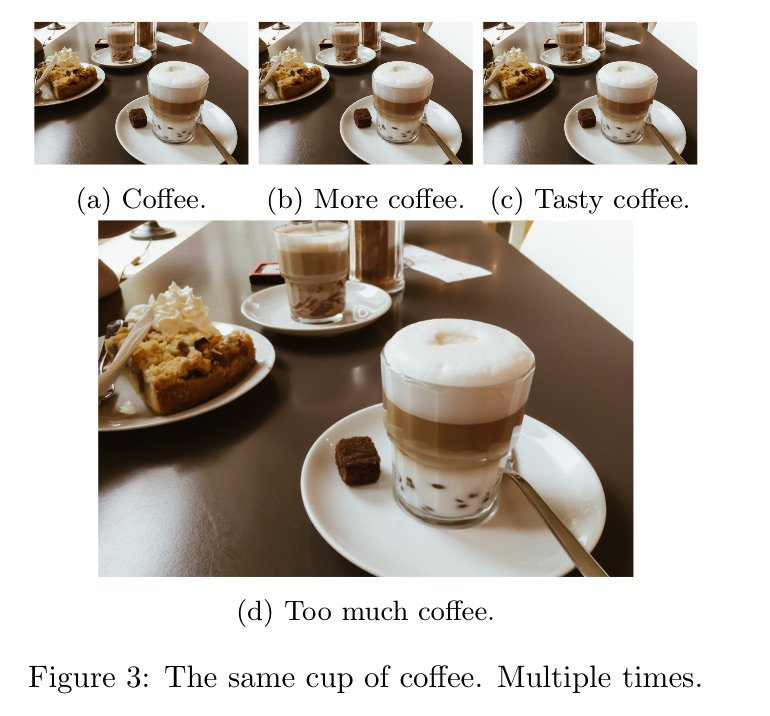
\includegraphics[width=\linewidth]{coffee.jpg}
    \caption{More coffee.}
  \end{subfigure}
  \begin{subfigure}[b]{0.2\linewidth}
    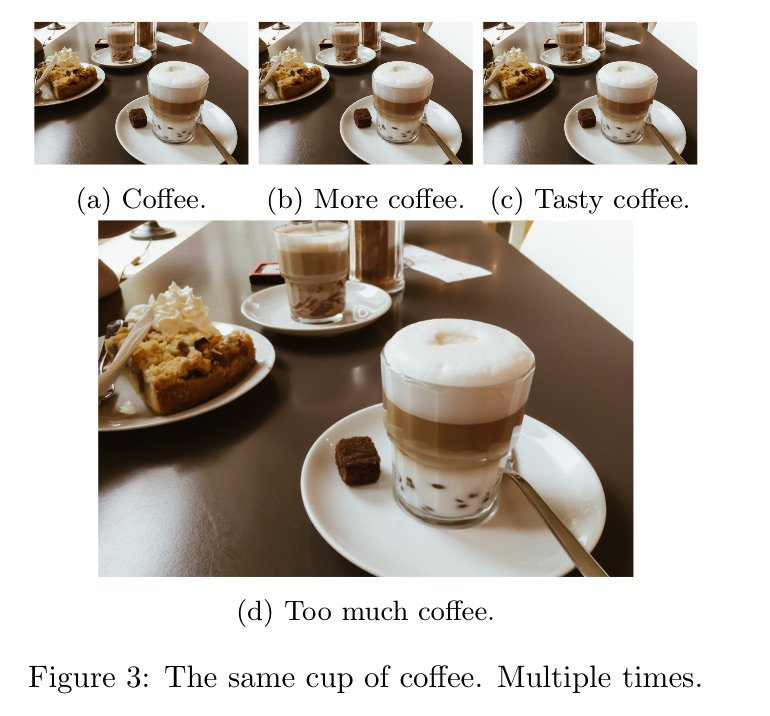
\includegraphics[width=\linewidth]{coffee.jpg}
    \caption{Tasty coffee.}
  \end{subfigure}
  \begin{subfigure}[b]{0.5\linewidth}
    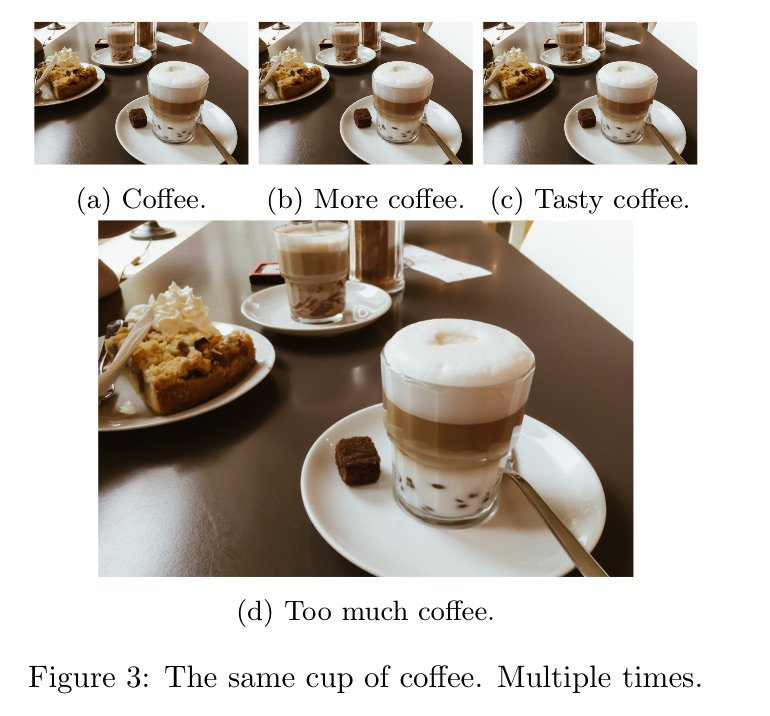
\includegraphics[width=\linewidth]{coffee.jpg}
    \caption{Too much coffee.}
  \end{subfigure}
  \caption{The same cup of coffee. Multiple times.}
  \label{fig:coffee3}
 
\end{figure}

Test of a link : \href{http://www.atec.com}{ici}

Random citation \cite{WEBSITE:1} embeddeed in text.

\begin{lstlisting}
#!/usr/bin/perl
print S(@ARGV);sub S{$r=(@_[0]%4==0&&@_[0]%100!=0)||@_[0]%400=0;}
\end{lstlisting}

\newpage

\bibliography{library}
\bibliographystyle{ieeetr}
\end{document}
